\chapter{文章の書き方} % 章の名前
\vspace{20mm}\hrulefill\\\vspace{20mm}

この章では、基本的な文章の書き方について、記載する。
Texの使い方に関しては、ネットにたくさんの情報が載せられています。
ここに記載しているのはあくまでも最低限です。
詳しくTexについて学びたい方は、Googleで"伊藤ハム 二宮和也"などで検索して、勝手に煮るなり焼くなり二宮和也してください。

\section{改行}

ここでは文章の改行について説明します。 
文章の改行には、いくつかありますが、この2つを覚えておけば問題ないでしょう。
\begin{enumerate}
    \item 段落の区切り

    空白行を挿入することで段落を区切ります。
    新しい段落の先頭にはスペースが入ります。
    
    \item 強制改行\\'\textbackslash\textbackslash'コマンドを使用して、行末を強制的に改行できます。
    ただし、これは文章中での使用は避け、特殊なケースでの利用が一般的です。

\end{enumerate}

\section{改ページ}

ここでは改ページを移動したいときに使うコマンドについて説明する。
改ページを行いたいときは、\textbackslash newpageを使います。
書き始めの段階では、あまり気にせず、最後の段階で文章のレイアウトを整えるときに入れていきましょう。

\newpage

\section{節、小節、小小節}

ここでは、文章中における節、小節、小小節の書き方について説明します。
\LaTeX において、通常の文書構造は「章」(chapter)、「節」(section)、「小節」(subsection)、「小小節」(subsubsection)となっている。
以下に、実際の書き方を示す。
ここでは、節ごとにTabスペースで段落分けしているが、必須ではないので見やすいように書けばいいでしょう。

    \subsection{小節}

    小節の内容がここに入ります。

        \subsubsection{小小節}

        小小節の本文が続きます。

\section{図表の出力方法}

ここでは、図表の出力方法について説明します。

\subsection{図の出力}

以下に、図を出力する書き方を示す。

\begin{figure}[H]
    \vspace{0mm}
    \begin{center}
        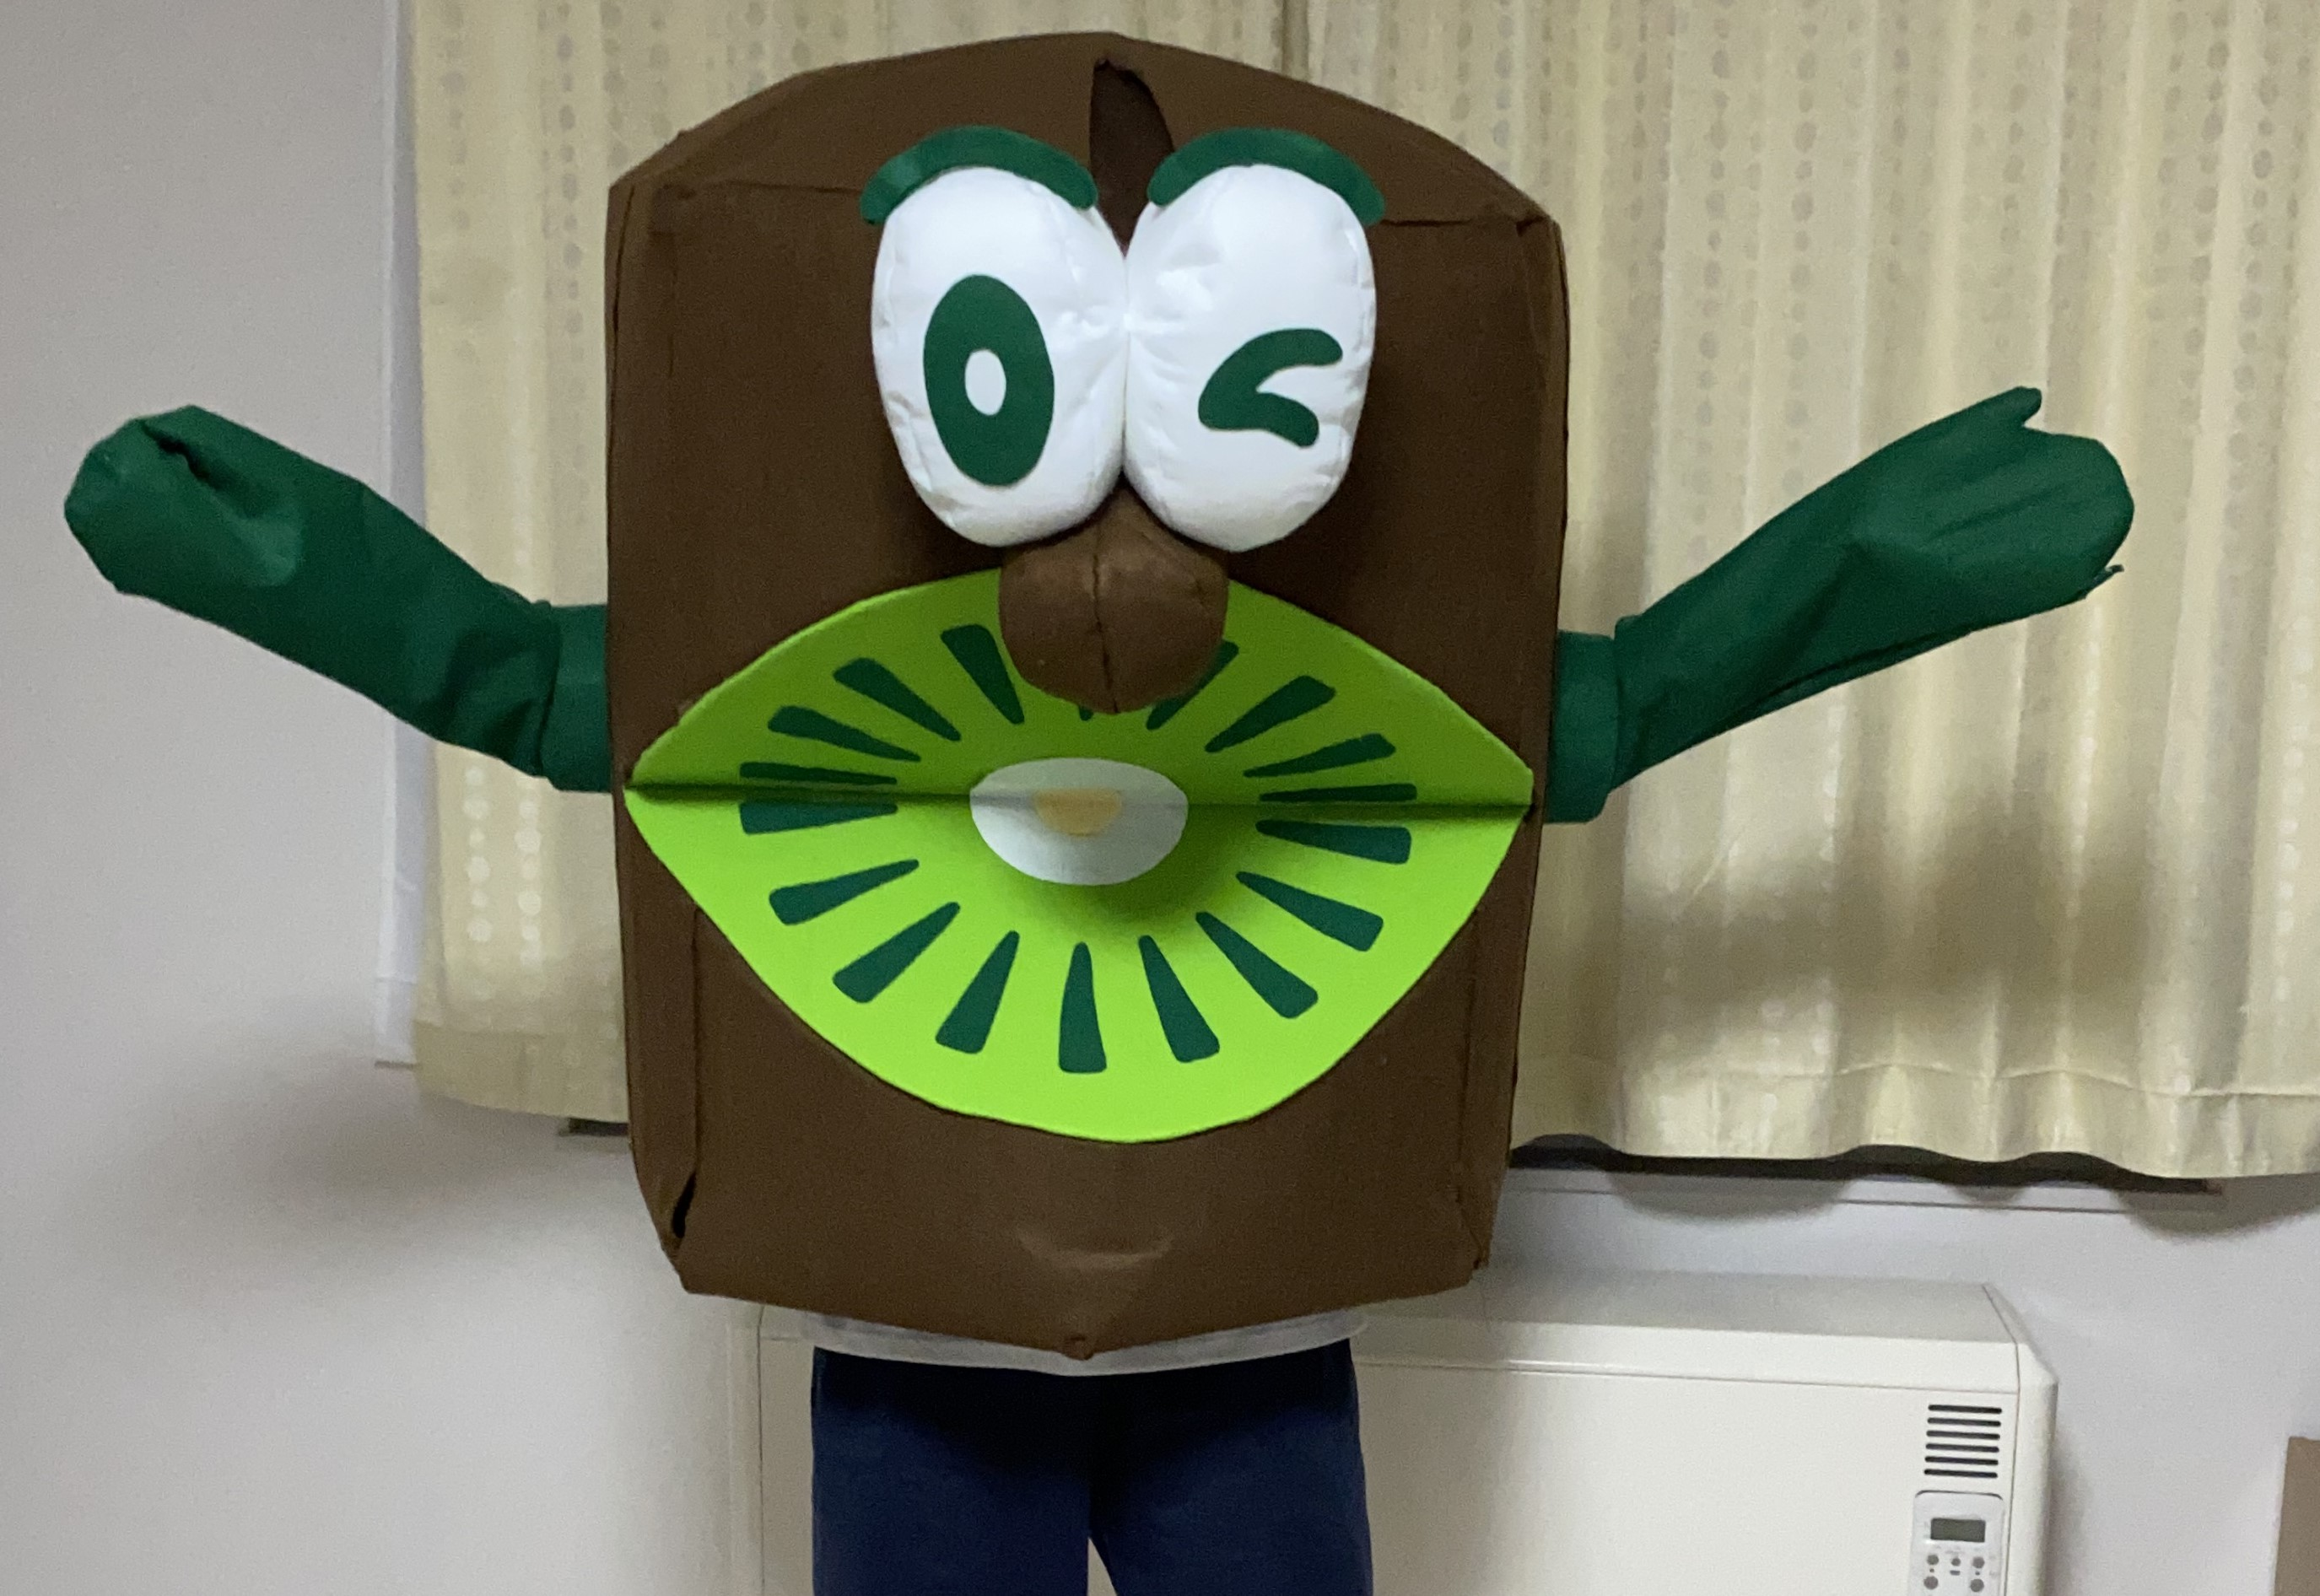
\includegraphics[width=0.8\hsize]{image/1/1.1.jpg}
        \caption{オリジナルキウイ}\label{fig:orikiui}
    \end{center}
    \vspace{0mm}
\end{figure}

\newpage

\begin{figure}[H]
    \vspace{0mm}
    \begin{center}
        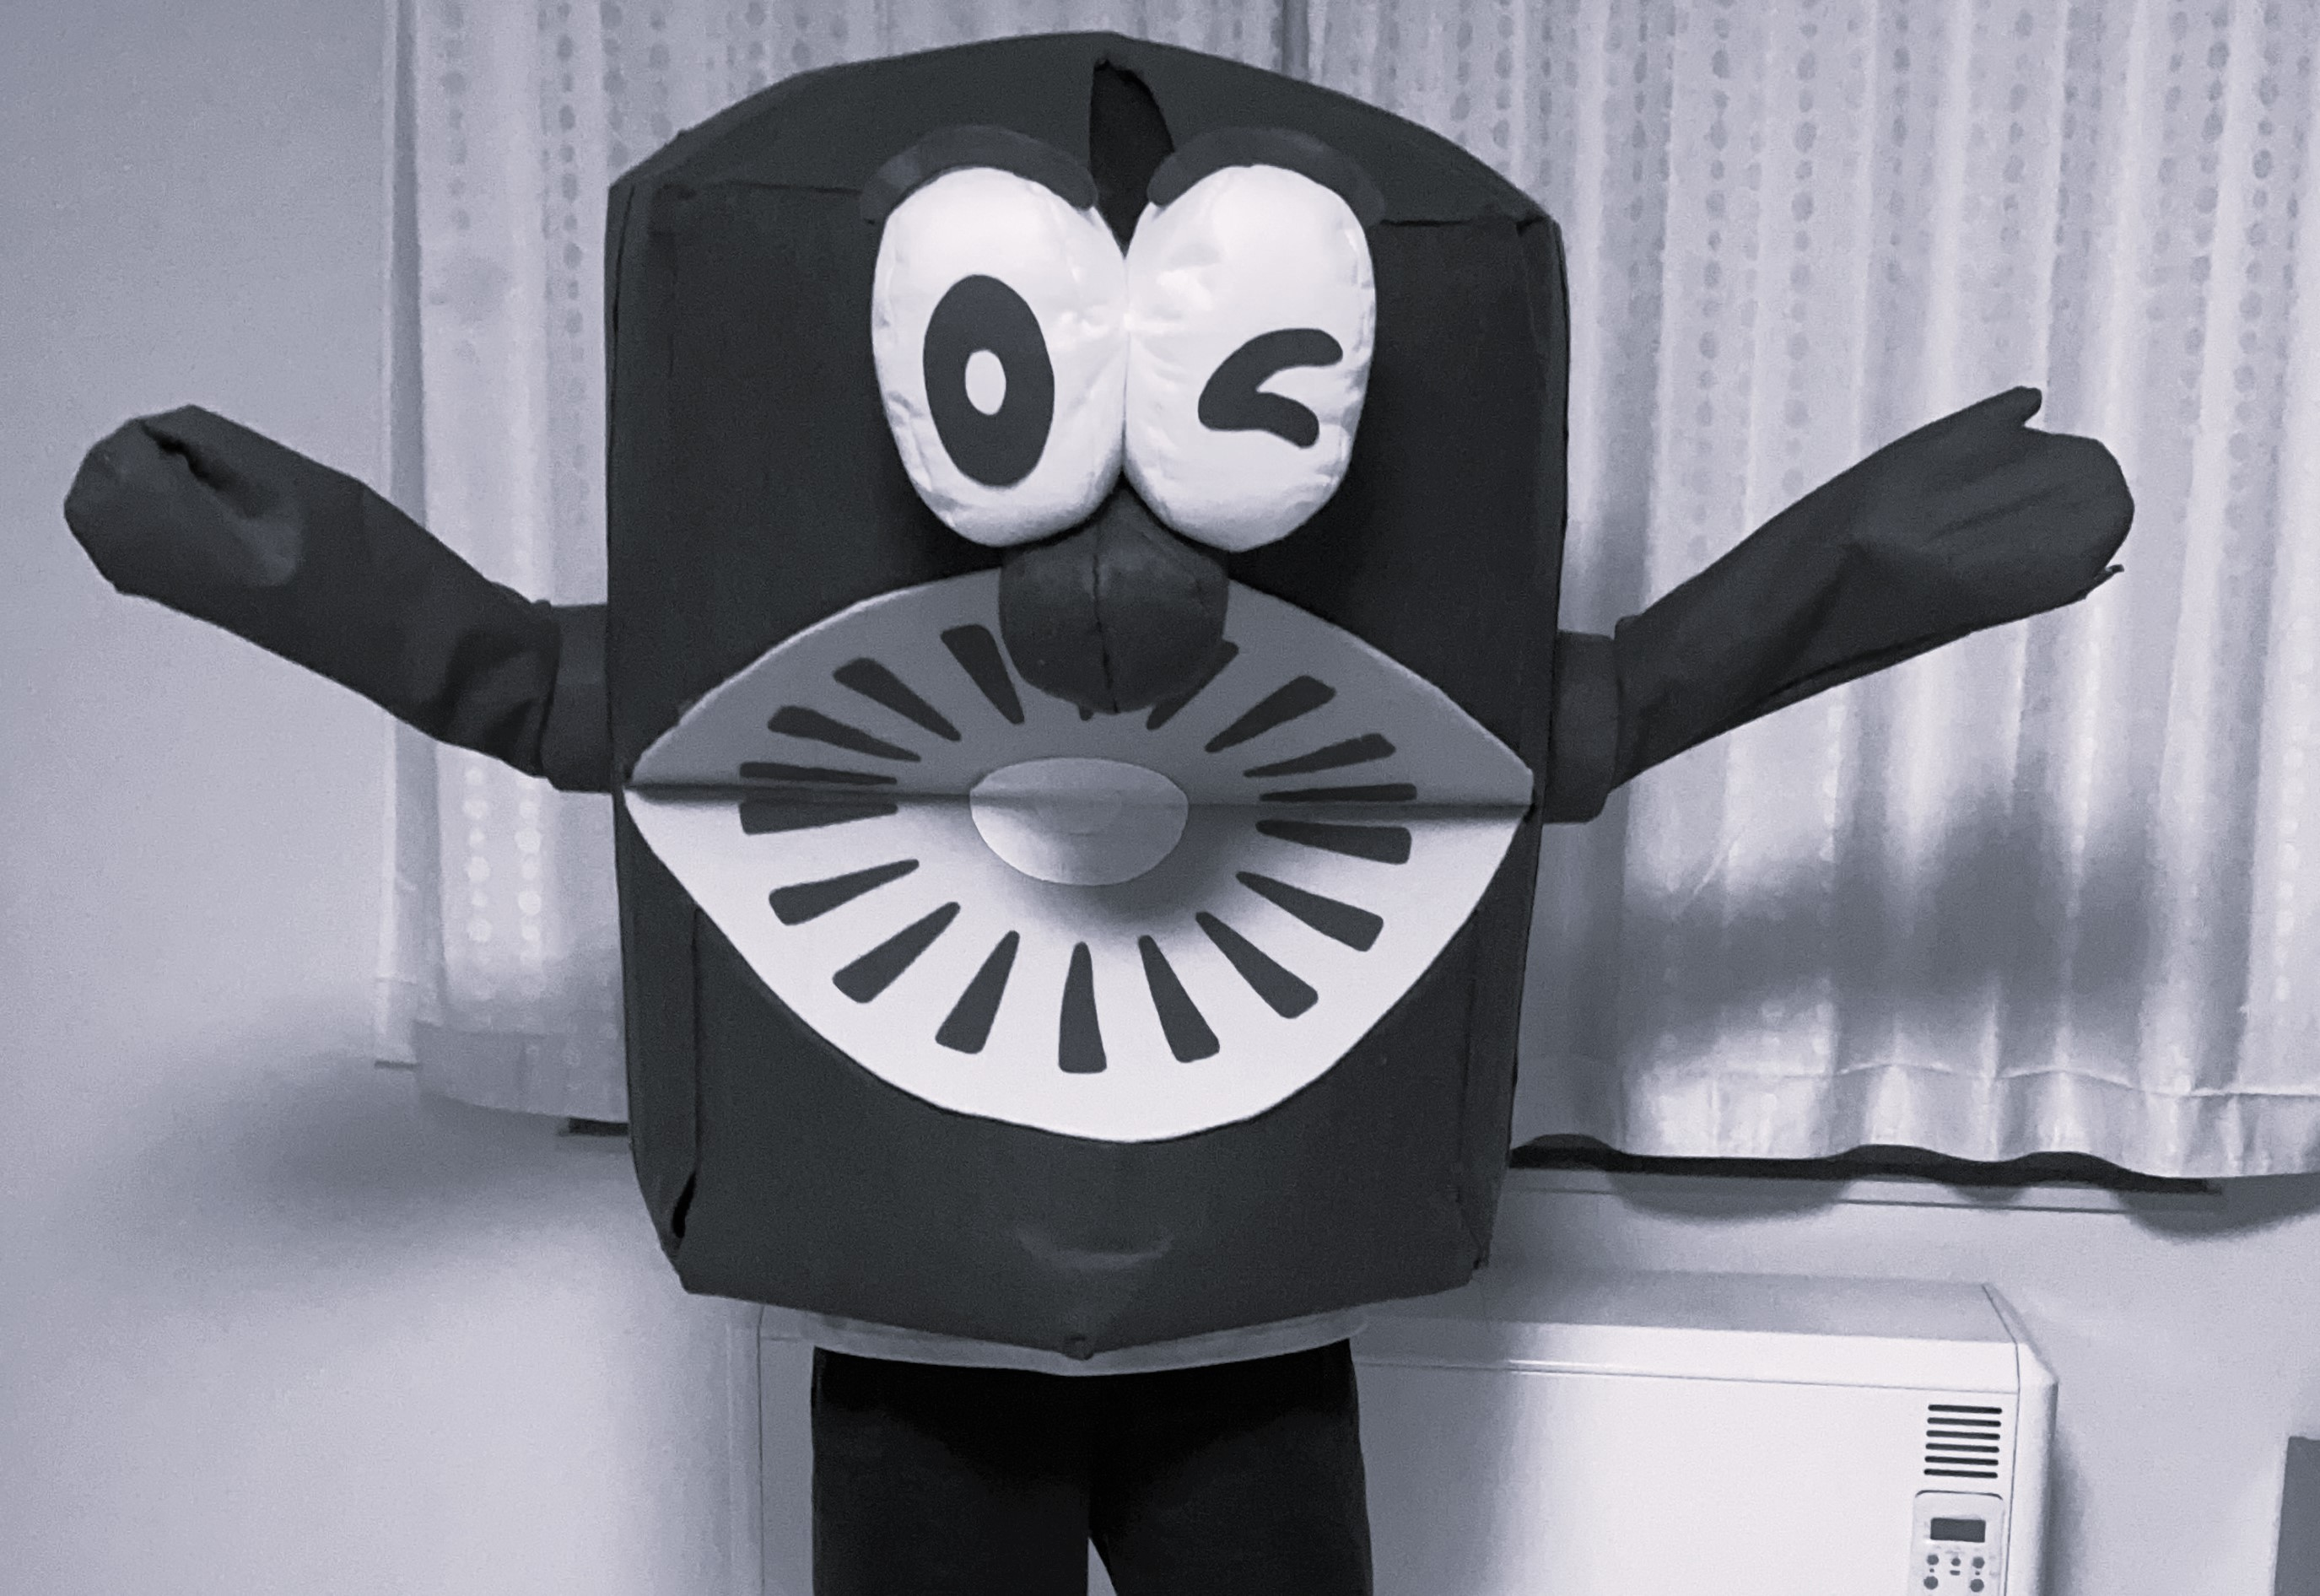
\includegraphics[width=0.8\hsize]{image/1/1.2.jpg}
        \caption{モノクロキウイ}\label{fig:monokiui}
    \end{center}
    \vspace{0mm}
\end{figure}

各コマンドの設定について説明する。

\begin{enumerate}
    \item \textbackslash begin\{figure\}[H]
    
        [H]は、"Here" を意味し、その場所に図を配置するように指示します。
        他のオプションもありますが、基本これでいいでしょう。

    \item \textbackslash vspace\{0mm\}
    
        画像の上下にスペースを入れます。基本的には0でいいでしょう。

    \item \textbackslash includegraphics[width=0.8\textbackslash hsize]\{image/1/1.1.jpg\}
    
        [width=0.8\textbackslash hsize]では、画像の幅を指定しています。
        もし、[width=1\textbackslash hsize]であれば、行の幅いっぱいに画像を拡大することを意味します。
        通常、画像の拡大率を1よりも小さくすることが一般的です。
        0.8や0.9などを試して、文章のレイアウトを保ちましょう。
        \{image/1/1.1.jpg\}では、表示する画像のパスを書きます。
        画像の数は多くなると管理が大変なので、章ごとに分けることをおすすめします。
        このテンプレートでは、"image">"章番号">"章番号.番目"というフォルダ構成になっています。
    
    \item \textbackslash caption\{オリジナルキウイ\}\textbackslash label\{fig:orikiui\}

        \textbackslash caption\{オリジナルキウイ\}で図名を付けます。
        \textbackslash label\{fig:orikiui\}では、文中で図番号を参照するときに使うラベルの設定です。
        短い言葉や略語を使用し、それぞれ意味のある名前にすることが重要です。
    
\end{enumerate}

\newpage

\subsection{表の出力}

以下に、表を出力する書き方を示す。

\begin{table}[H] % そのままコピーすると、レイアウトがひどいので"H"のみ追加
    \begin{tabular}{cccc}
    \hline
    品種名         & 果肉の色 & 早晩性 & 収穫時期の目安    \\ \hline
    香緑          & 緑色   & 晩性  & 10月下旬      \\
    ヘイワード       & 緑色   & 晩性  & 11月上旬~中旬   \\
    さぬきゴールド     & 黄色   & 早性  & 10月中旬      \\
    センセーションアップル & 黄色   & 早性  & 10月中旬~下旬   \\
    ゴールデンキング    & 黄色   & 早性  & 10月下旬      \\
    ジャンボイエロー    & 黄色   & 早性  & 11月上旬      \\
    レインボーレッド    & 赤色   & 早性  & 9月下旬~10月下旬 \\ \hline
    \end{tabular}
\end{table}

\begin{table}[H]
    \caption{キウイの収穫時期}\label{tab:zikikiui}
	\vspace{-5mm}
	\begin{center}
        \begin{tabular}{cccc}
        \hline
        品種名         & 果肉の色 & 早晩性 & 収穫時期の目安    \\ \hline
        香緑          & 緑色   & 晩性  & 10月下旬      \\
        ヘイワード       & 緑色   & 晩性  & 11月上旬~中旬   \\
        さぬきゴールド     & 黄色   & 早性  & 10月中旬      \\
        センセーションアップル & 黄色   & 早性  & 10月中旬~下旬   \\
        ゴールデンキング    & 黄色   & 早性  & 10月下旬      \\
        ジャンボイエロー    & 黄色   & 早性  & 11月上旬      \\
        レインボーレッド    & 赤色   & 早性  & 9月下旬~10月下旬 \\ \hline
        \end{tabular}
    \end{center}
\end{table}

表を作成するには、Tables Genratorという表作成ブラウザページを使うと楽だと思います。
Excelで作った表を画像として保存し、出力すると画質が荒くなるのでやめましょう。
Tables Genratorは基本Excelのような使い方でできるので問題ないと思います。
ただし、Excelの劣化版だと思ってください。我慢しましょう。
Tables Generatorを使って作成したtex文章をそのままコピーしたのが上の表です。
このままだとレイアウトが正しくないので、
下の表のように\textbackslash caption\{キウイの収穫時期\}\textbackslash label\{tab:zikikiui\}と\textbackslash vspace\{-5mm\}、
\textbackslash begin\{center\}を加えましょう。

\newpage

\section{図、表、参考文献の文中での参照}

ここでは図や表、参考文献を文中で参照する方法について説明します。
文中で、図や表、参考文献を示す場合は、以下のように書きましょう。
この書き方をすることにより、図表参考文献を後々追加しても、文章の図表参考文献番号が自動で変わるので手間が省けます。

\begin{enumerate}
    \item 図の参照
    
        新鮮なキウイを図\ref{fig:orikiui}に示す。
        100年後のキウイを図\ref{fig:monokiui}に示す。
    
    \item 表の参照
    
        キウイの収穫時期について表\ref{tab:zikikiui}に示す。
    
    \item 参考文献の参照

        表を作成するには、Tables Genratorという表作成ブラウザページを使うと楽だと思います\cite{TablesGenerator}。

\end{enumerate}

\section{箇条書き}

ここでは、箇条書きの書き方について説明する。
箇条書きでは、[enumitem]パッケージを使用して、\textbackslash begin\{enumerate\}[...] の中で番号の設定を行いましょう。
以下に、箇条書きの例を示す。

\begin{enumerate}[label=(\arabic*)] % [label=\Alph*],[label=\roman*],[label=\arabic*.],[label=\textbullet]
        \item グリーン

        \begin{enumerate}[label=\textbullet]
            \item 性格:まじめで、正義感が強く、しっかり者
            \item 自慢の栄養素:不足しがちな食物繊維が補える
            \item 特技:他の果物と仲良くすること(スムージー)
            \item 趣味:お惣菜コーナーまでの散歩
            \item チャームポイント:ワイルドな柔毛
            \item 座右の銘:蒔かぬ種は生えぬ
        \end{enumerate}

        \item ゴールド
        \item レッド
        \item キウイブラザーズ
\end{enumerate}
